% --------------------
\mysec{Kreise}\bigskip
% --------------------
\begin{minipage}[c]{0.30\textwidth}
  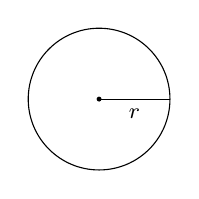
\begin{tikzpicture}[scale=0.9]
    \draw (0, 0) circle (1cm);
    \draw (0, 0) -- node[below]{{\footnotesize$r$}} (1, 0);
    \fill (0, 0) circle (1pt);
  \end{tikzpicture}
\end{minipage}%
\begin{minipage}[c]{0.70\textwidth}
  \formrow{U=2\pi r}
  \formrow{A=\pi r^{2}}\vspace*{-\bigskipamount}
\end{minipage}\bigskip

Kreisbogen:\medskip\par
\begin{minipage}[c]{0.30\textwidth}
  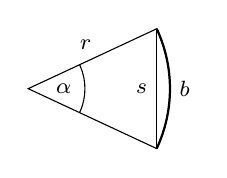
\begin{tikzpicture}[scale=0.9]
    \node[shift=(115:2mm)] at (25:1cm) {{\footnotesize$r$}};
    \node[right] at (2, 0) {{\footnotesize$b$}};
    % Winkel
    \begin{scope}
      \clip (0, 0) -- (-25:2cm) arc (-25:25:2cm) -- cycle;
      \draw (0, 0) circle (8mm);
      \node at (0:5mm) {{\footnotesize$\alpha$}};
    \end{scope}
    % Sehne
    \draw (-25:2cm) -- node[left]{{\footnotesize$s$}}(25:2cm);
    \draw (0, 0) -- (-25:2cm) arc (-25:25:2cm) -- cycle;
    \draw[line width=0.8pt] (-25:2cm) arc (-25:25:2cm);
  \end{tikzpicture}
\end{minipage}%
\begin{minipage}[c]{0.70\textwidth}
  \formrow{b=\frac{\pi\alpha}{180}\cdot r}
  \formrow{s=2r\cdot\sin\frac{\alpha}{2}}\vspace*{-\bigskipamount}
\end{minipage}\bigskip

Kreisausschnitt:\medskip\par
\begin{minipage}[c]{0.30\textwidth}
  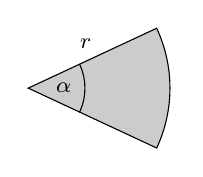
\begin{tikzpicture}[scale=0.9]
    \node[shift=(115:2mm)] at (25:1cm) {{\footnotesize$r$}};
    % Flaeche
    \fill[fill=white!80!black] (0, 0) -- (-25:2cm) arc (-25:25:2cm) -- cycle;
    % Winkel
    \begin{scope}
      \clip (0, 0) -- (-25:2cm) arc (-25:25:2cm) -- cycle;
      \draw (0, 0) circle (8mm);
      \node at (0:5mm) {{\footnotesize$\alpha$}};
    \end{scope}
    \draw (0, 0) -- (-25:2cm) arc (-25:25:2cm) -- cycle;
  \end{tikzpicture}
\end{minipage}%
\begin{minipage}[c]{0.70\textwidth}
  \formrow{A=\frac{\pi\alpha}{360}\cdot r^{2}}\vspace*{-\bigskipamount}
\end{minipage}\bigskip

Kreisabschnitt:\medskip\par
\begin{minipage}[c]{0.30\textwidth}
  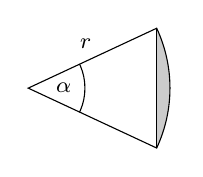
\begin{tikzpicture}[scale=0.9]
    \node[shift=(115:2mm)] at (25:1cm) {{\footnotesize$r$}};
    % Flaeche
    \fill[fill=white!80!black] (-25:2cm) arc (-25:25:2cm) -- cycle;
    % Winkel
    \begin{scope}
      \clip (0, 0) -- (-25:2cm) arc (-25:25:2cm) -- cycle;
      \draw (0, 0) circle (8mm);
      \node at (0:5mm) {{\footnotesize$\alpha$}};
    \end{scope}
    \draw (0, 0) -- (-25:2cm) arc (-25:25:2cm) -- cycle;
    % Sehne
    \draw (-25:2cm) -- (25:2cm);
  \end{tikzpicture}
\end{minipage}%
\begin{minipage}[c]{0.70\textwidth}
  \formrow{A=\frac{r^{2}}{2}\cdot\left(\frac{\pi\alpha}{180}-\sin\alpha\right)}\vspace*{-\bigskipamount}
\end{minipage}

